\section*{Die Newtonschen Axiome}

Bisher haben wir uns mit der Statik beschäftigt. In der Statik ist die Summe aller
an einen Körper angreifenden Kräfte Null. Ausserdem verschwinden alle Drehmomente bezüglich
einer beliebigen Drehachse. Ist eine dieser Bedingungen nicht erfüllt, bewegt sich der Körper.

%Bewegungen haben wir in der Kinematik untersucht.

Ausserdem haben wir die Bewegung eines Körpers durch Ort, Geschwindigkeit und Beschleunigung
beschrieben (Kinematik). Im folgenden Abschnitt wollen wir lernen \emph{warum} ein Körper sich bewegt.
Diese Gebiet der Physik wird als Dynamik bezeichnet.
Isaac Newton hat im Jahre 1686 drei Grundgesetze (Axiome) aufgestellt, die bis heute die Grundlage
der klassischen Mechanik bilden.

%Eine fundamentale Rolle in den Newtonschen Axiomen spielt die Kraft $F$.
%Die physikalische Kraft $\vec{F}$ ist eine vektorielle Grösse. Man kennt sie erst,
%wenn ihr Betrag, ihre Richtung und ihr Angriffspunkt bekannt sind. Die Einheit
%der Kraft heisst Newton.
%Eine Kraft kann man nicht direkt sehen. Wenn Gegenstände verformt werden, wie zum Beispiel
%eine Metallfeder verlängert oder gestaucht wird, dann wirken Kräfte.
%Auch wenn es zur Beschleunigung eines Gegenstands kommt sind Kräfte nötig.

Mit den folgenden Versuchen wollen wir die Newtonschen Axiome kennenlernen und
selber reproduzieren:

\subsection*{Experiment: Luftkissenbahn}

\begin{figure}[h!]
\begin{center}

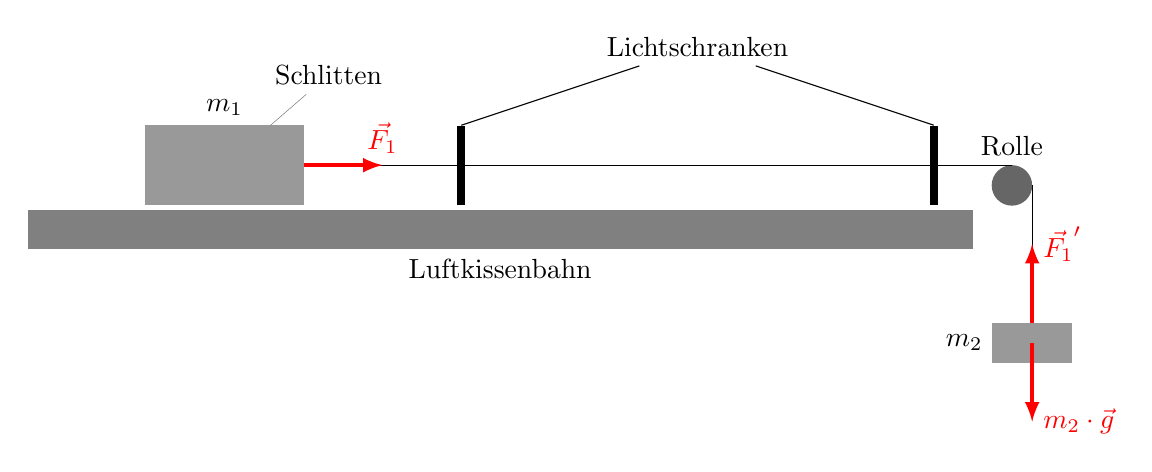
\begin{tikzpicture}
%\begin{tikzpicture}
%\usetikzlibrary{calc,intersections,through,backgrounds}
%\usetikzlibrary{decorations.pathmorphing}
%\draw[step=0.5cm,lightgray] (-0.5,-3.0) grid (6.5,5.0);
\usepgflibrary{arrows}
\tikzset{force/.style={>=latex,line width=0.05cm}}
%\newcommand{\RI}[2]{\ensuremath{#1_{\textrm{#2}}}}

\draw (5,0) node [minimum height=0.5cm, minimum width=12cm, fill, color=black!50,label=below:Luftkissenbahn] (B) {}; %bahn

\draw (B.north)+(-3.5cm,0.05cm) node [anchor=south,minimum height=1cm, minimum width=2cm,draw,fill, color=black!40, label=above:$m_1$,pin= 60:Schlitten] (M1) {}; %wagen

\draw (M1) +(10cm,0) node[anchor=north,circle,minimum size=0.5cm,draw,fill, color=black!60, label=above:Rolle] (R) {}; %rolle

\draw (R.east)+(0,-2cm) node[minimum height=0.5cm,minimum width=1cm,draw,label=left:$m_2$,fill,color=black!40] (M2) {}; %angehängtes gewicht

%\draw (M2.south)+(0,-1.2cm) node[minimum width=2cm, minimum height=0.1cm,anchor=north,fill,color=black!60, label=below:Tisch] (T){}; %Tisch

\draw (M1.east)--(R.north) (R.east)--(M2.north); %faden

%Kräfte
\draw [->,color=red,force] (M2.center)--+(-90:1cm) node [right] {$m_2\cdot \vec{g}$};
\draw[->,color=red,force] (M2.north)--+(90:1cm) node [right] {$\vec{F_1}'$};
\draw[->,color=red,force] (M1.east)--+(0:1cm) node [above]{$\vec{F_1}$};

 %Lichtschranke1}
\draw (M1.east)+(2cm,0) node[inner sep=0,minimum width=0.1cm,minimum height=1cm,fill] (L1){}; %Lichtschranke1

\draw (L1)+(6cm,0) node[inner sep=0,minimum width=0.1cm,minimum height=1cm,fill] (L2){}; %Lichtschranke1

\draw (L1.north)+(3cm,1.0cm) node (LL) {Lichtschranken};
\draw (LL)--(L1.north);
\draw (LL)--(L2.north);

\end{tikzpicture}

\end{center}
\caption{\label{fig:luftkissen} Luftkissenbahn}
\end{figure}


In folgenden wollen wir ein Experiment durchführen.
Der Versuchsaufbau ist in Abbildung~\ref{fig:luftkissen} skizziert. Ein Schlitten gleitet reibungsfrei
auf einer Luftkissenbahn. 
%Teil 1 ohne Masse m2
Im ersten Versuchsteil fehlt die Masse $m_2$. Ist der Schlitten
in Ruhe, so bleibt er an seiner Position. Hat der Schlitten eine von Null verschiedene Geschwindigkeit,
so behält er diese bei. Dies haben wir auch schon früher einmal gesehen.
Dieses Verhalten wird im ersten Newtonschen Axiom behandelt: Das Trägheitsgesetz.

\begin{cbox}
	\textbf{Das Trägheitsgesetz}\\
	``Ein Körper verharrt im Zustand der Ruhe oder der gleichförmigen Translation, sofern er nicht durch einwirkende Kräfte zur Änderung seines Zustands gezwungen wird.''\\oder im lateinischen Original:\\
	``Corpus omne perseverare in statu suo quiescendi vel movendi uniformiter in directum, nisi quatenus illud a viribus impressis cogitur statum suum mutare.''
\end{cbox}

%Teil 2 mit Masse m2
Im zweiten Versuchsaufbau verbinden wir den Schlitten mit einem Faden mit der Masse $m_2$
und untersuchen, wie sich der Bewegungszustand des Schlittens dadurch verändert.

%\newpage

\newcommand\lZIIII{\phantom{x} & \phantom{x} & \phantom{x} & \phantom{x}\\\hline}
\begin{center}
%\begin{large}
	\begin{tabular}{p{0.18\textwidth}|p{0.18\textwidth}||p{0.25\textwidth}p{0.25\textwidth}}
		\multicolumn{2}{c}{Messwerte} & \multicolumn{2}{c}{Auswertung}\\ 
    Masse $m_2$ (kg) & $\Delta t$ (s) & & \\\hline
	\lZIIII
	\lZIIII
	\lZIIII
	\lZIIII
	\lZIIII
	\lZIIII
	\lZIIII
	\lZIIII
	\end{tabular}
%\end{large}
\end{center}

\begin{aufgabe}
	\label{Fma}
	\begin{enumerate}[a)]
		\item	Beschreiben Sie den Versuch mit eigenen Worten.
		\item Werten Sie die Messwerte aus. Von Interesse sind die auf den Schlitten wirkende Kraft und die Beschleunigung des Schlittens.
		\item Tragen Sie die ausgewerteten Daten in ein Diagramm ein.
		\item Was haben Sie herausgefunden?
	\end{enumerate}
\end{aufgabe}

\newpage

\begin{cbox}\label{newton2}
	\textbf{Das Aktionsprinzip}\\
``Die Änderung der Bewegung ist der Einwirkung der bewegenden Kraft proportional und geschieht nach der Richtung derjenigen geraden Linie, nach welcher jene Kraft wirkt.''
	\\oder im lateinischen Original:\\
``Mutationem motus proportionalem esse vi motrici impressae, et fieri secundum lineam rectam qua vis illa imprimitur.''
\end{cbox}

Bekannter als diese ausformulierte Variante des zweiten Newtonschen Axioms ist die dazu gehörige Formel:
\begin{eqnarray*}
	F=m\cdot a\text{.}
\end{eqnarray*}
$F$ ist die auf einen Gegenstand wirkende Kraft, $m$ ist dessen Masse und $a$ ist die von der Kraft $F$ verursachte Beschleunigung des Körpers.
Im letzten Experiment (siehe Aufgabe \ref{Fma}) haben wir dieses Gesetz in dieser Form bestätigt.

\Einbinden{\dir/newton01.tex}
\Einbinden{\dir/newton02.tex}
\Einbinden{\dir/newton03.tex}



